% Asset ID: AS1AlgebraicMethodsProofTikZ-002
% Source: CCEA proof/reasoning theme + Chapter 7b transcript
% Related lesson section: Big Picture Explanation; Core Theory; Exam Technique
% Purpose: Decision tree for choosing proof by deduction, proof by exhaustion or disproof by counterexample.

\documentclass[tikz,border=8pt]{standalone}
\usepackage{amsmath}
\usetikzlibrary{arrows.meta,positioning,shapes.geometric}
\begin{document}
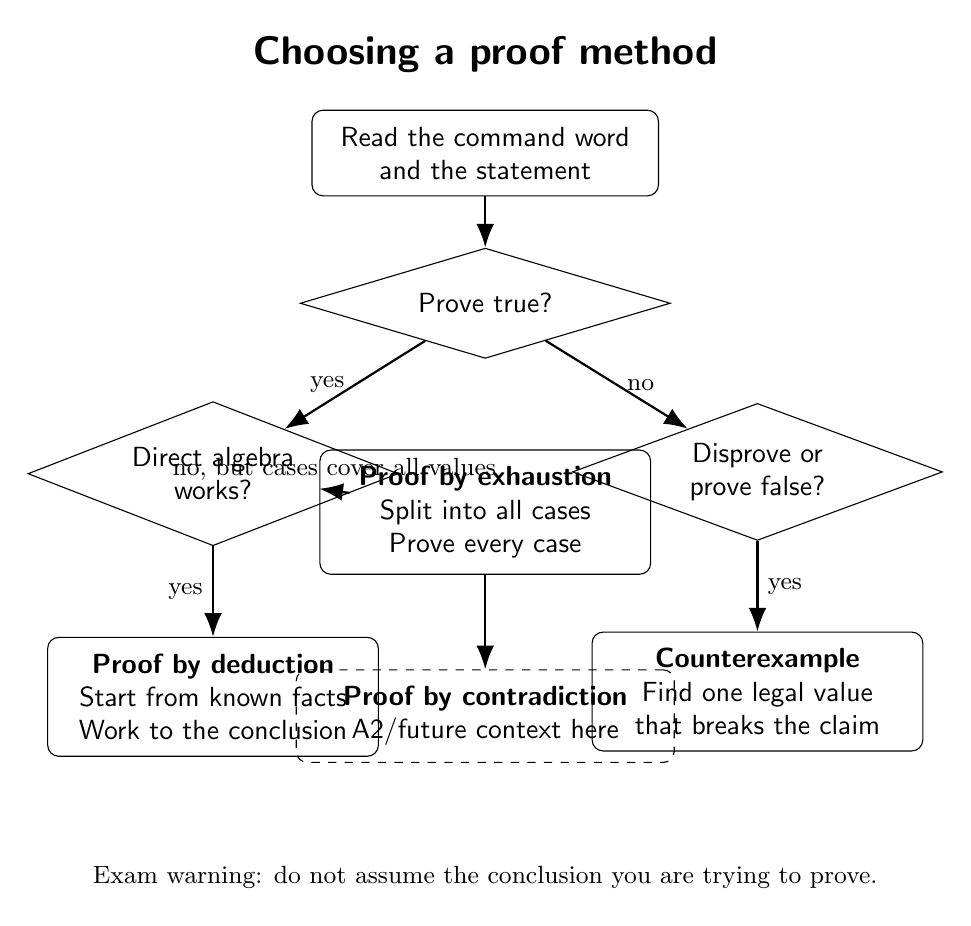
\begin{tikzpicture}[font=\sffamily,node distance=1.25cm,start/.style={draw,rounded corners,align=center,minimum width=4.4cm,minimum height=1cm,inner sep=6pt},decision/.style={draw,diamond,aspect=2.15,align=center,inner sep=2pt,minimum width=4.7cm,minimum height=1.4cm},method/.style={draw,rounded corners,align=center,minimum width=4.2cm,minimum height=1.45cm,inner sep=6pt},future/.style={draw,dashed,rounded corners,align=center,minimum width=4.8cm,minimum height=1.15cm,inner sep=6pt},arr/.style={-{Latex[length=3mm]}, thick}]
\node[font=\sffamily\bfseries\Large, align=center] (title) at (0,5.2){Choosing a proof method};
\node[start] (start) at (0,3.95){Read the command word\\and the statement};
\node[decision, below=0.65cm of start] (true){Prove true?};
\node[decision, below left=1.35cm and 1.1cm of true] (direct){Direct algebra\\works?};
\node[decision, below right=1.35cm and 1.1cm of true] (false){Disprove or\\prove false?};
\node[method, below=1.15cm of direct] (deduction){\textbf{Proof by deduction}\\Start from known facts\\Work to the conclusion};
\node[method, below=1.15cm of true] (exhaustion){\textbf{Proof by exhaustion}\\Split into all cases\\Prove every case};
\node[method, below=1.15cm of false] (counter){\textbf{Counterexample}\\Find one legal value\\that breaks the claim};
\node[future, below=1.2cm of exhaustion] (contradiction){\textbf{Proof by contradiction}\\A2/future context here};
\draw[arr] (start) -- (true);\draw[arr] (true) -- node[left, font=\small] {yes} (direct);\draw[arr] (true) -- node[right, font=\small] {no} (false);\draw[arr] (direct) -- node[left, font=\small] {yes} (deduction);\draw[arr] (direct) -- node[above, font=\small] {no, but cases cover all values} (exhaustion);\draw[arr] (false) -- node[right, font=\small] {yes} (counter);\draw[arr] (exhaustion) -- (contradiction);
\node[align=center, font=\small] at (0,-5.25){Exam warning: do not assume the conclusion you are trying to prove.};
\end{tikzpicture}
\end{document}
